\subsubsection{Struktura danych chromosomu}
\begin{par}
	Jeśli chodzi o typ struktury danych przyjęto pierwszy schemat (rys.\ref{fig:sterowanie}), wraz z krzyżowaniem statystycznym. 
	O ile ukierunkowanie systemu na gry jednego typu może lepiej się sprawdzić jeśli zależy nam
	jedynie na szybkim i optymalnym wyniku, to generalizacja systemu i elastyczna implementacja całego algorytmu da nam lepsze narzędzie nie tylko dydaktyczne, ale też badawcze.
	Przykładem może być popularna gra Galaxian. Sama definicja klawiszy w Galaxian i Super Mario Brothers jest podobna (klawisze kierunkowe + klawisze specjalne),
	jednak schemat poruszania się jest już inny: O ile gry typu Mario Brothers pasują do powyższych założeń o kierunkowości ruchu, to w grze Galaxian już tak nie jest.
	Korzystniej zatem jest traktowanie projektu jako systemu rozwiązującego gry platformowe czasu rzeczywistego na podstawie przyciśnięć klawiszy w czasie.
\end{par}
\begin{par}
	
	Sam chromosom przechowuje następujące dane:

	\begin{itemize}
		\item Tablicę dotyczącą akcji ruchu przechowującą wartości typu wyliczeniowego: UP,DOWN,LEFT,RIGHT,NONE
		\item Tablicę dotyczącą akcji specjalnych: A,B,C,D,NONE
		\item Instancję obiektu \textit{ResultData} przechowującego dane dotyczące wyniku funkcji przystosowania, oraz wartości ustalane po przetestowaniu danego chromosomu takie jak czas który upłynął, rodzaj wyniku, ilość zebranych punktów.
	\end{itemize}

	Wartość NONE w obu tablicach odpowiada za brak akcji. 
	Wartości A,B,C,D odpowiadają za kolejne klawisze specjalne które mogą być traktowane przez środowisko gry jako skok lub strzał. 
	Ograniczamy się do 4 klawiszy specjalnych, które wystarczają w zupełności do zrealizowania większości gier platformowych.

	Oprócz tego każdy Chromosom uzupełnia interfejs Comparable, dzięki czemu obiekty mogą być porównywane ze sobą. Porównanie składa się jedynie z porównania wyniku wartości funkcji przystosowania. Dzięki temu możemy łatwo posortować całe populacje.
	Obiekt ten przechowuje dane na temat wyniku danego chromosomu i danych pomocniczych, które sa uzupełniane po przetestowaniu chromosomu. 
	Oprócz tego chromosom posiada metody pozwalające na mutację zarówno tablicy ruchu jak i tablicy akcji specjalnych.
\end{par}
\subsubsection{Dane konfiguracyjne}
\begin{par}
	Jak już zostało wspomniane, podstawą dobrego systemu, szczególnie do zastosowań badawczych jest łatwo dostępna konfiguracja. 
	W pracy rolę tę pełni pośrednio klasa \textit{GeneticsConfig} która zawiera wszystkie najważniejsze parametry dotyczące algorytmu (takie jak prawdopodobieństwo mutacji) są przechowywane jako wartości tablicy asocjacyjnej (klasa \textit{JHashMap}). 
	Oprócz tego sama tablica została opakowana w taki sposób iż rejestracja nowej wartości do tablicy wiąże się z automatycznym wygenerowaniem odpowiedniego pola w panelu konfiguracyjnym. 
	Dzięki temu mamy pewność iż wszystkie parametry biorące udział w algorytmie będą w pełni konfigurowalne.
\end{par}
\begin{par}
	Każda z akcji, zarówno ruchu jak i specjalna posiada prawdopodobieństwo wystąpienia.
	Wartości te również dostępne są w panelu konfiguracyjnym, przy czym są one normalizowane do sumy wszystkich wartości z danej kategorii.
	Przykładowo dla wartości podanych na rys \ref{fig:config1}. Wartość ruchu w prawo (grupa ``Movement key probabilities'') wynosi $\frac{2.5}{2.5+0.5+0.2}=0.78125$.
	\begin{figure}[!h]
		\centering
		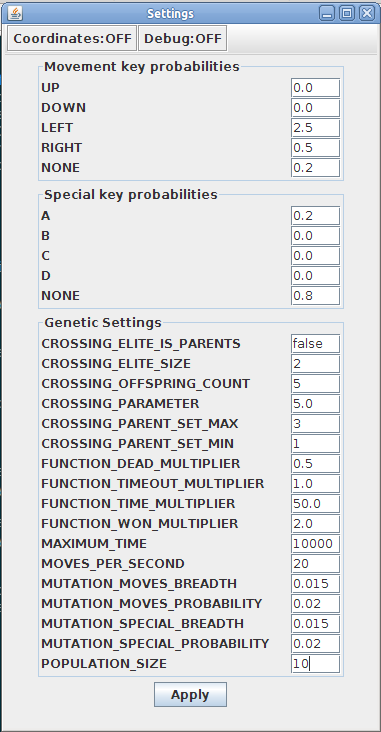
\includegraphics[width=2in]{obrazki/config1.png}
		\caption{Panel Konfiguracyjny.}
		\label{fig:config1}
	\end{figure}
	Oprócz tego klasa GeneticsConfig posiada metody pozwalające na zwrócenie losowej akcji w zależności od prawdopodobieństwa jej wystąpienia - rys \ref{fig:config1}.
\end{par}

